\documentclass[a4paper,10pt,fullpage]{article}
\usepackage[utf8]{inputenc}
\usepackage[english]{babel}
\usepackage[a4paper]{geometry}		
\geometry{top=1.5cm, bottom=1cm, left=2cm, right=1.5cm} 	
\usepackage{hyperref}
\usepackage{enumitem}
\usepackage{graphicx}
\usepackage{wrapfig}
%\graphicspath{ {./images/} }
\pagenumbering{gobble}
\setlength{\parindent}{0em}


% % % % % % % % % % % % % % % % % % % % % % % % % % % % % % % % % % % % %
\begin{document}
\setlist{nolistsep}

% % % % % % % % % % % % % % % % % % % % % % % % % % % % % % % % % % % % %

\begin{wrapfigure}{l}{0.21\textwidth}
	%\centering
	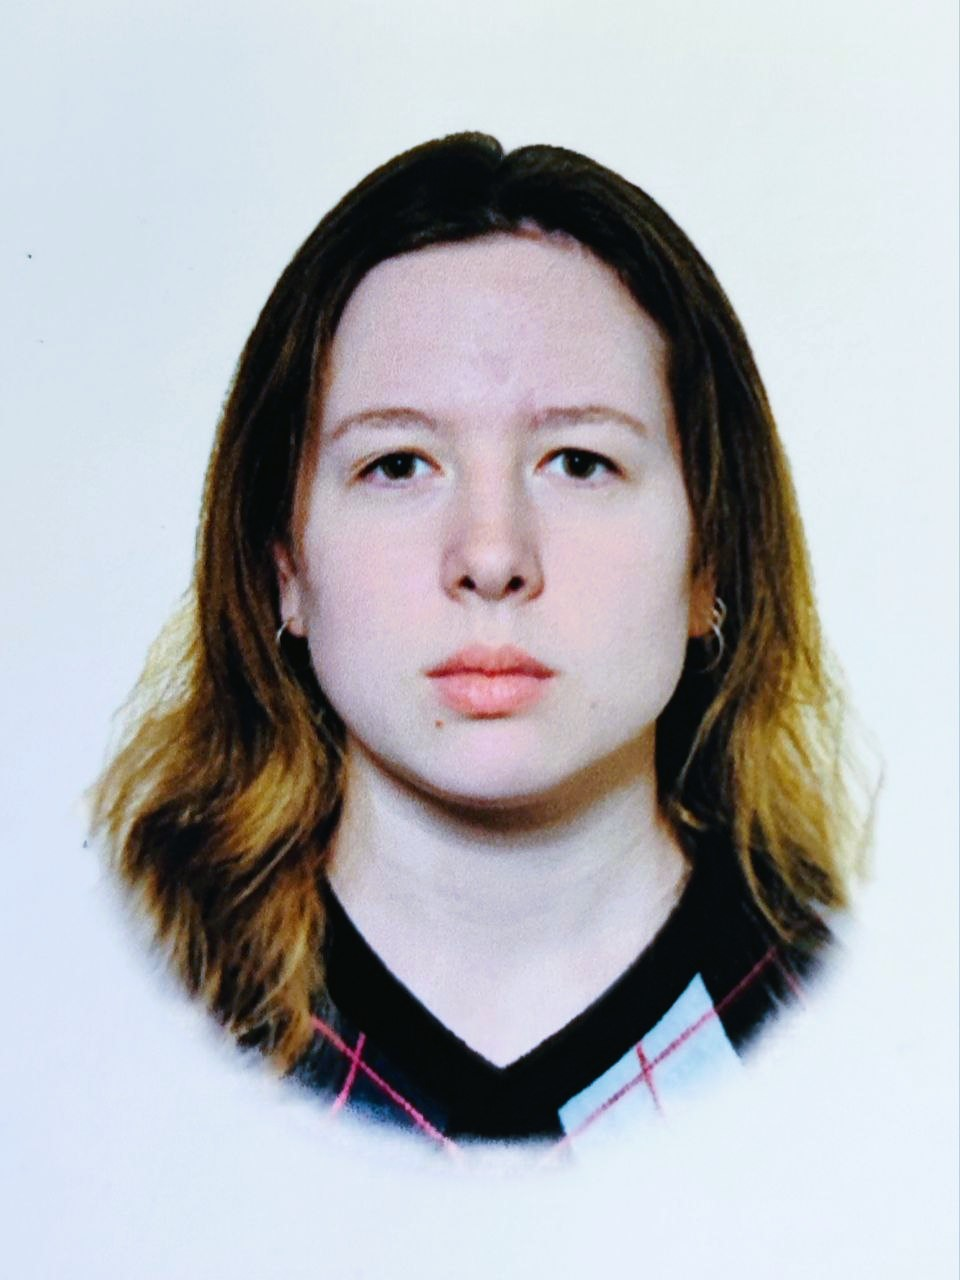
\includegraphics[width=0.21\textwidth]{photo1}
\end{wrapfigure}

\underline{\textbf{\LARGE Svetlana Golubeva}}\\

\underline{Contacts:} lana.a.golubeva@gmail.com, Cel: +39 342 7996584, LinkedIn: \href{https://www.linkedin.com/in/lana-golubeva/}{lana-golubeva}. \\
\underline{Birth Date:} October 26, 1989.\\
\underline{Residence:} Lipomo(CO), Italia. %Eligible to work in Europe.\\


% % % % % % % % % % % % % % % % % % % % % % % % % % % % % % % % % % % % %
\begin{center}
	\underline{\textbf{\large Competenze:}}
\end{center}
\underline{Programming Languages}: Python, C/C++.\\
\underline{OS}: Windows, Linux (Debian, Void, Slackware, LFS).\\
\underline{Other}: SQL, Git, \LaTeX, TiKz, UML, BPM, Emacs, Notion.\\
\underline{Fields}: Networks and System Administration, Data Analysis e Machine Learning, Process Automation, Microelectronics.\\
\underline{Languages:} Russian (native), Italian (advanced), English (advanced). \\


% % % % % % % % % % % % % % % % % % % % % % % % % % % % % % % % % % % % %
\begin{center}
	\underline{\textbf{\large Working Experience:}}
\end{center}	

\textbf{Como Luxury Suites} Como, Italy (2 years 11 month).\\
\underline{Receptionist}, July 2023 -- ...
\begin{itemize}
	\item[--] Client and suppliers relations.	
	\item[--] Continuous analysis of financial data, prognosis and updates on growth strategies.\\
\end{itemize}

\textbf{Business Intelligence and Data Analysis  Consultant} (5 years and 4 month).\\
\underline{Freelance}, September 2017 -- December 2022.
\begin{itemize}
	\item[--] Digital Transformation, automation and optimization of business processes.\\
\end{itemize}

\textbf{A' Design Award \& Competition} Como, Italy (5 years 3 month).\\
\underline{Logistics Manager}, May 2019 -- November 2021.
\begin{itemize}
	\item[--] Optimization of shipment preparation and post-processing.
	\item[--] Management of package assembly line.
\end{itemize}
\underline{Logistics Specialist}, September 2017 -- April 2019.
\begin{itemize}	
	\item[--] Management and optimization of shipment preparation and processing. 
	\item[--] Planning and preparation of Gala Events and exhibitions set-up.
\end{itemize}
\underline{System Administrator}, September 2016 -- August 2017.
\begin{itemize}
	\item[--] System Administration and infrastructure improvement.\\
\end{itemize}


\textbf{Moscow State Institute of Radio Engineering, Electronics and Automation (MIREA)} Moscow, Russia (6 years).\\
\underline{Senior Tecnical Consultant}, September 2015 -- August 2017.
\begin{itemize}
	\item[--] Project management and supervision for graduating students.
	\item[--] Development of the conceptual architecture of the search system for the department portal.
	\item[--] Integration of Machine Learning methods into current scientific research.
	\item[--] Development of a concept for monitoring of suspicious activity based on user behavioral patterns in IoT networks.
\end{itemize}
\underline{Tecnical Consultant}, September 2013 -- August 2015.
\begin{itemize}
	\item[--] Transfer of the departmental infrastructure to Open Source Software.
	\item[--] Development of the architecture for department's educational and administrative portal.
\end{itemize}
\underline{Tecnical Consultant}, September 2011 -- August 2013.
\begin{itemize}
	\item[--] Management of the department network and computer laboratories.
	\item[--] Teacing assistance.
\end{itemize}


% % % % % % % % % % % % % % % % % % % % % % % % % % % % % % % % % % % % %
\begin{center}
	\underline{\textbf{\large Education:}}
\end{center}	
\textbf{Politecnico di Milano}, Como, Italia.\\
2013 - 2016 -- Master Courses in Computer Science (academic exchange program, double degree.)\\

\textbf{Moscow State Institute of Radio Engineering, Electronics and Automation (MIREA)}, Moscow,
Russia.\\
2013 - 2015 -- M.Sc. in Computer Scientce -- Artificial Intelligence, Natural Language Processing.\\
2011 - 2013 -- Advanced training / second degree -- translator in the field of science, engineering and technology.\\
2009 - 2013 -- B.Sc. in Computer Scientce -- Artificial Intelligence.


% % % % % % % % % % % % % % % % % % % % % % % % % % % % % % % % % % % % %
\begin{center}
\underline{\textbf{\large Certificates:}}
\end{center}	
\textbf{Stanford University}, Lagunita MOOC.\\
2016 --- Statistical Learning.


% % % % % % % % % % % % % % % % % % % % % % % % % % % % % % % % % % % % %
\vfill

\hline
\vspace{3pt}
\scriptsize Autorizzo il trattamento dei miei dati personali presenti nel curriculum vitae ai sensi del Decreto Legislativo 30 giugno 2003, n. 196 e del GDPR (Regolamento UE 2016/679).

% % % % % % % % % % % % % % % % % % % % % % % % % % % % % % % % % % % % %
\end{document}
